La construcción mecánica del brazo robótico esta basada en impresión 3D en material PLA.
De esta forma, tres motores paso a paso se encargan de mover, mediante  engranajes, el brazo
en los tres ejes. Como cabezal se implemento una pinza accionada por un servo motor.
\par
Como microcontrolador se utilizo el Atmega328p, además de tres drives Unl2003 encargados del control de los motores paso a paso.
\par
Tanto el código para el microcontrolador, como el programa de consola para la PC, fue implementado en C en su totalidad.
Sin embargo, la interfaz gráfica para la PC, fue desarrollada en C++ por medio del entorno de programación QtCreator.
\begin{figure}[!htb]
  \begin{center}
    \subfloat[]{{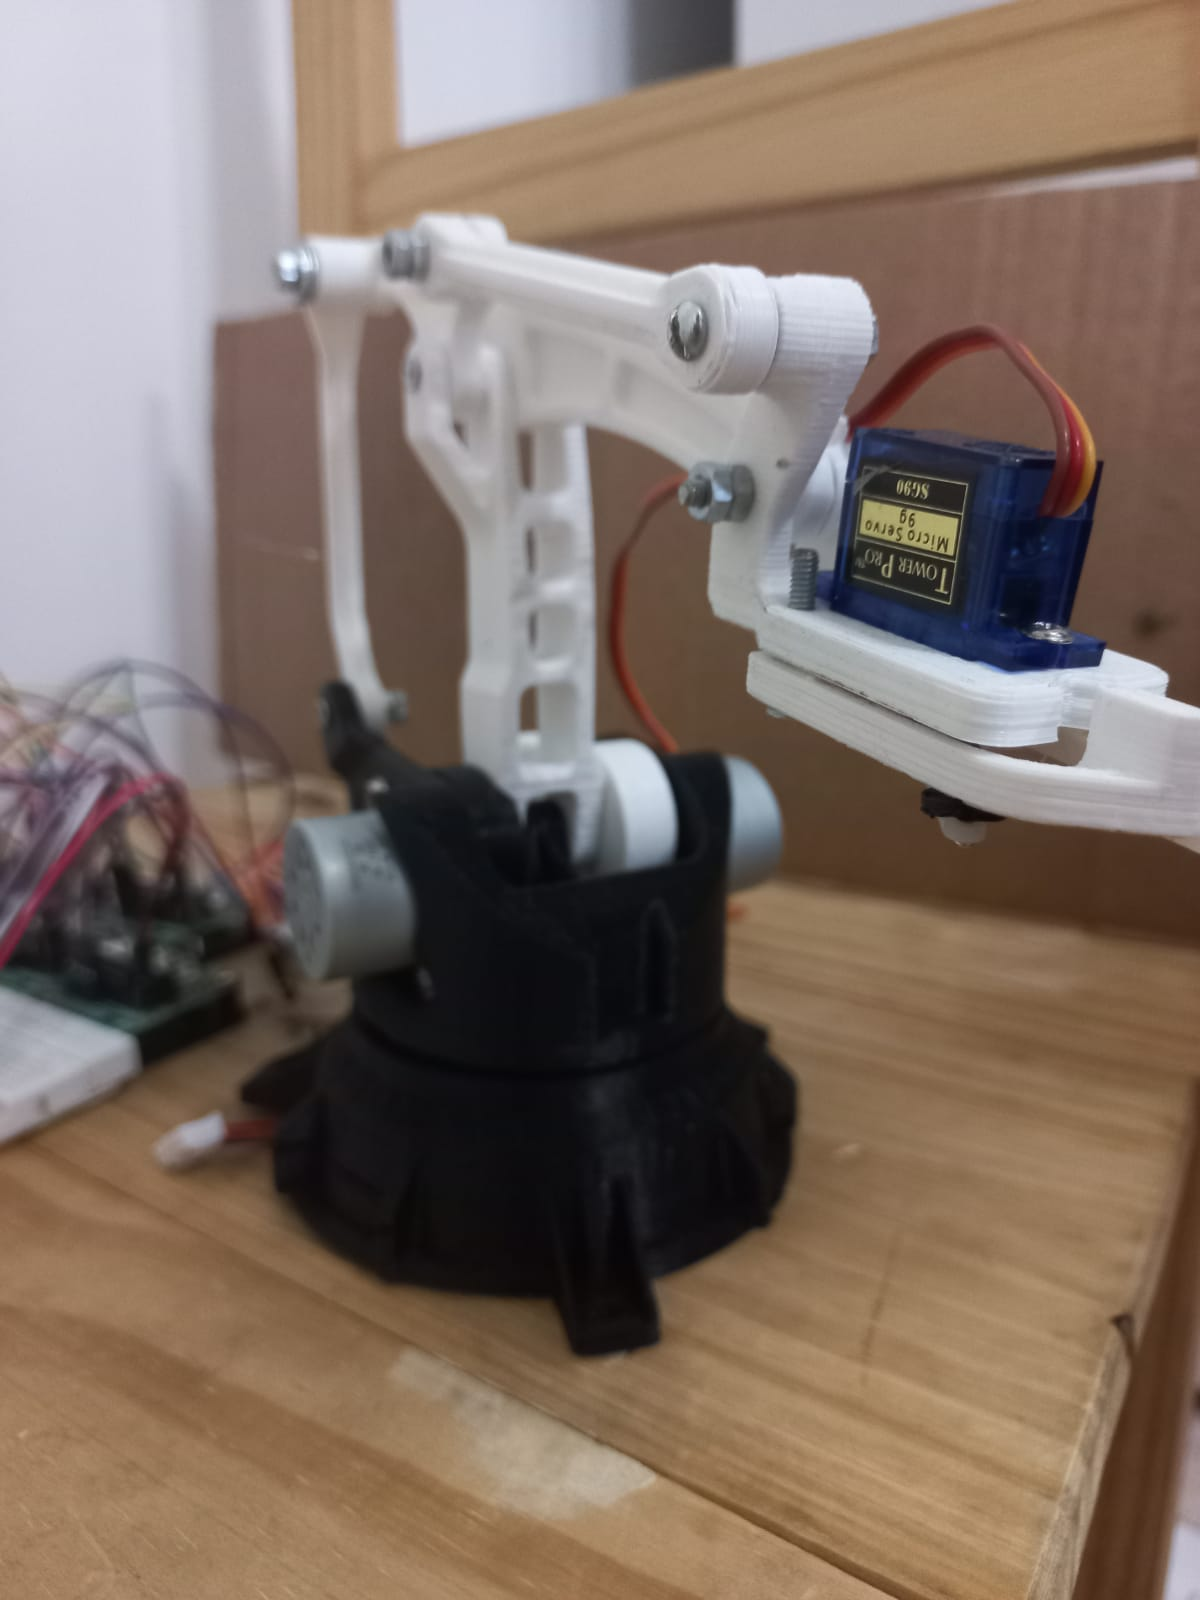
\includegraphics[width=6cm]{imagenes/Brazo1.jpeg} }}%
    \qquad
    \subfloat[]{{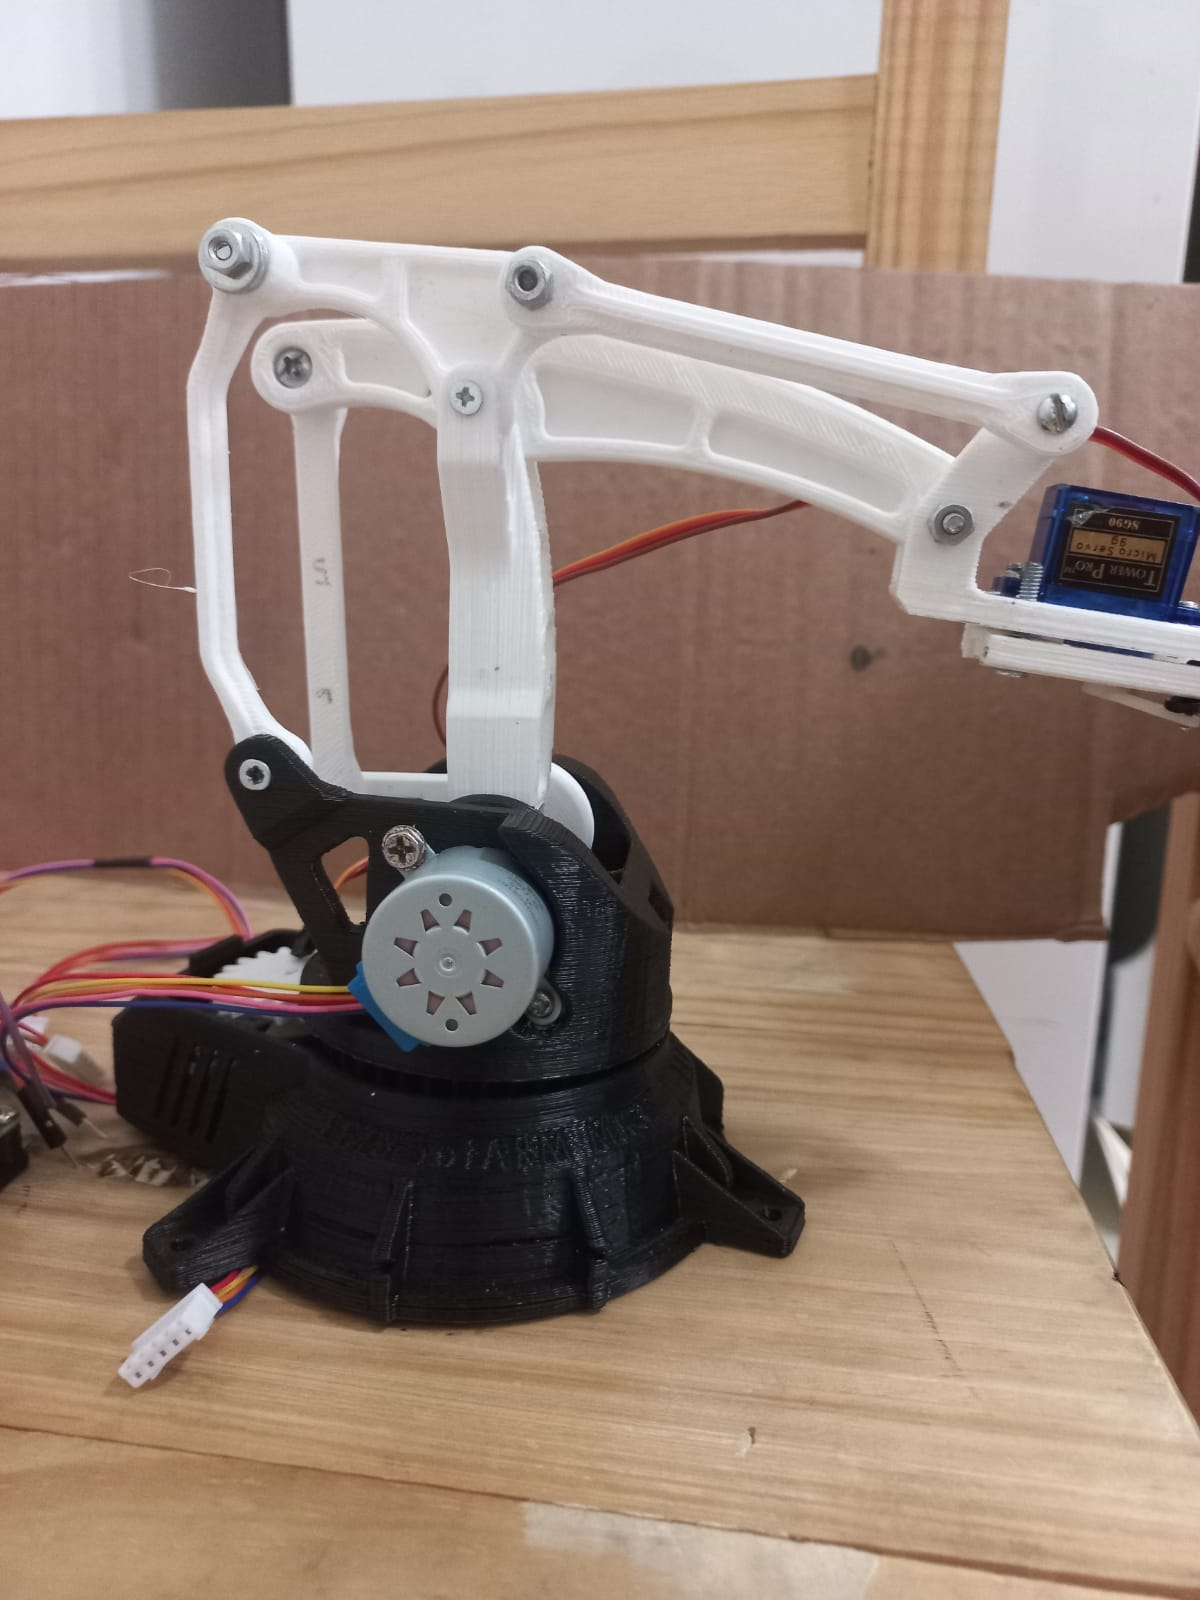
\includegraphics[width=6cm]{imagenes/Brazo2.jpeg} }}%
  \end{center}
  \caption{Imagen del brazo robótico}
  \label{fig:brazo}
\end{figure}
